\section{Purpose}
 

\section{Method}

\section{Results}
For the implementation of the “Da Vinci surgical system” in the Operating theatre simulation a Cyclic Coordinate Descent (CCD) Inverse Kinematic (IK) method is used. The IK finds values for all connected joints so that an end-effector reaches a desired position and orientation. Chin et al [1] compares different solutions to the IK problem. CCD is an optimisation method for minimising a nonlinear cost function. The method iterates through a list of variables and adjusts the values to minimise the cost. The use of CCD to solve the IK problem is documented by Wang and Chen [2]. CCD iterates through all joints one at a time starting from the outermost one. For each joint an angle is chosen which moves the end-effector closest to the desired position.
\begin{figure}[h]
\centering
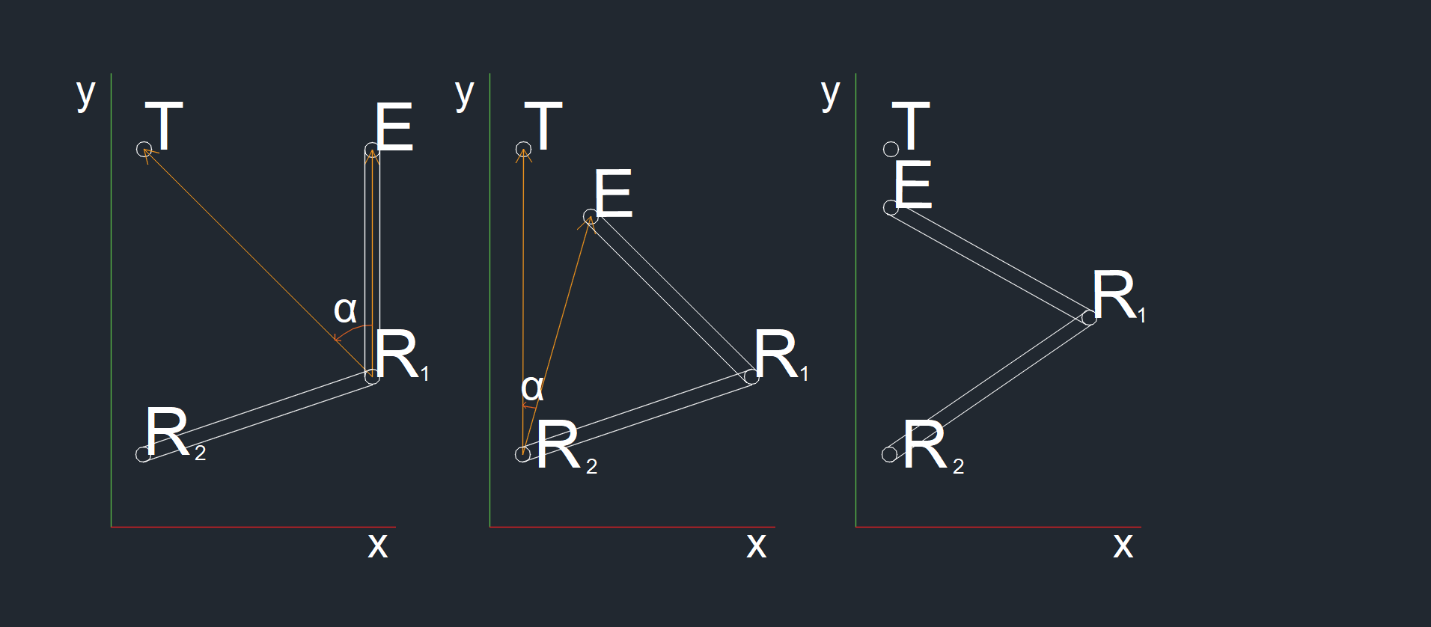
\includegraphics[scale=1]{CCD/IKCCD.png}
\caption{Visual example of IK using CCD }
\end{figure}
Figure 1 Visual example of IK using CCD (add more creative caption)
In Figure 1, a desired position T, end-effector position E and position of the current joint R1 calculating the rotation for R1 is achieved by calculating the dot product R1 $dot{T,R1}$ E and the cross product R1 $T*R1$ E, in both cases the vectors should be normalised. Using inverse cosine, it is possible to get the angle between the two vectors, and the cross product is used to show the direction in which the root needs to be rotated. In 2D the direction of the cross product is used, however in 3D the normalised cross product vector is multiplied by the angle between the two vectors providing three new angles, for each of the three axes respectively. Those angles are directly added to the current rotation of the root joint. This process is repeated for each joint in the list.

One addition to the algorithm is the implementation of a restriction vector. The restriction is a unit vector (for example [0,0,1]), when multiplied by the new rotation vector it effectively removes any rotation from two of the axes, allowing rotation to happen only around one. This allows for more realistic movement by not allowing joints to rotate in unnatural ways.
 \begin{figure}[h]
 \centering
 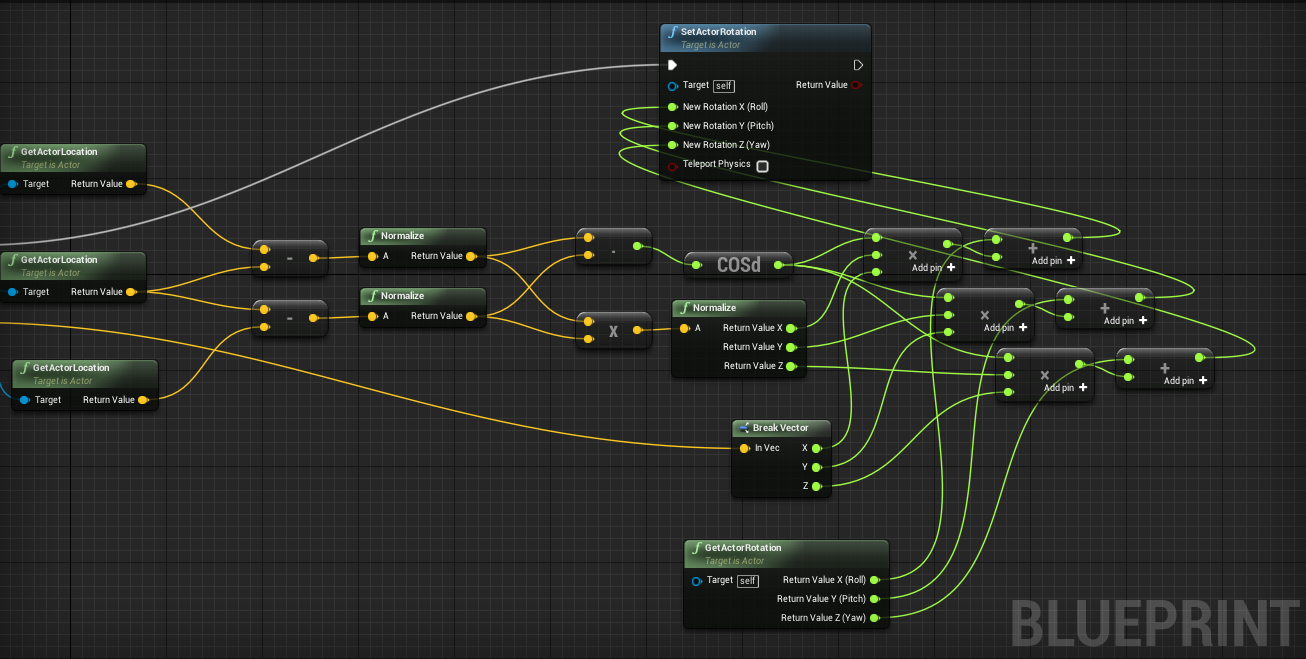
\includegraphics[scale=1]{CCD/CCDBlueprint.png}
 \caption{Blueprint that changes the rotation of object to position the end-effector closest to the desired position}
 \end{figure}
 
Figure 2 Blueprint that changes the rotation of object to position the end-effector closest to the desired position.
Because Unreal engine does not allow for easy manipulation of dedicated bone structures in real time a hierarchical joint system was used instead. Each joint share a parent child relationship with other joints in the chain, any changes made to the transform of a parent joint affects all of its children.


[1] K. W. Chin, B. R. von Konsky and A. Marriott, “Closed-form and generalized inverse kinematics solutions for the analysis of human motion,” Int. Conf. IEEE Eng. Med. Bio. Soc. 5, 1911–1914 (1997).
[2] L.-C. T. Wang and C. C. Chen, “A combined optimization method for solving the inverse kinematics problems of mechanical manipulators,” IEEE Trans. Robot. Autom. 7, 489– 499 (1991).



\section{Conclusion}
